\chapter{Números (1º Bimestre)}

\section{Conjuntos numéricos e sequências}

\subsection*{Conjuntos numéricos}

In the 1º Bimestre of the 8ª série do Ensino Fundamental, we discussed some
conjuntos numéricos. Os números reais (designoados por $\mathbb R$) podem ser
representados como pontos em uma reta.

\begin{center}
\begin{tikzpicture}
  \draw (-3,0) --(3,0);
  \path (-4,0) node (minf) {$\ldots$};
  \path (4,0) node (inf) {$\ldots$};
  \draw (-1,-.1) --(-1,.1);
  \draw (-2,-.1) --(-2,.1);
  \draw (0,-.1) --(0,.1);
  \draw (1,-.1) --(1,.1);
  \draw (2,-.1) --(2,.1);
  \path (0,.5) node (n0) {$0$};
  \path (1,.5) node (n1) {$1$};
  \path (2,.5) node (n2) {$2$};
  \path (-1,.5) node (nm1) {$-1$};
  \path (-2,.5) node (nm2) {$-2$};
\end{tikzpicture}
\end{center}

Os números naturais (designados por $\mathbb N$) são $0, 1, 2, 3, \ldots$. Se
também incluirmos os números negativos, obteremos os números inteiros
(designados por $\mathbb Z$: $\ldots, -3, -2, -1, 0, 1, 2, 3, \ldots$).
Os números da forma $\frac{p}{q}$ onde $p \in \mathbb Z$ e $q \in \mathbb N
\setminus \{0\}$ são chamados de racionais (designados por $\mathbb Q$). Em
particular, se considerarmos os números decimais onde $q = 10^n$ para algum $n
\in \mathbb N$, obteremos os números decimais como $-494.1627$.
Os reais que não são racionais são chamados de irracionais.

\begin{center}
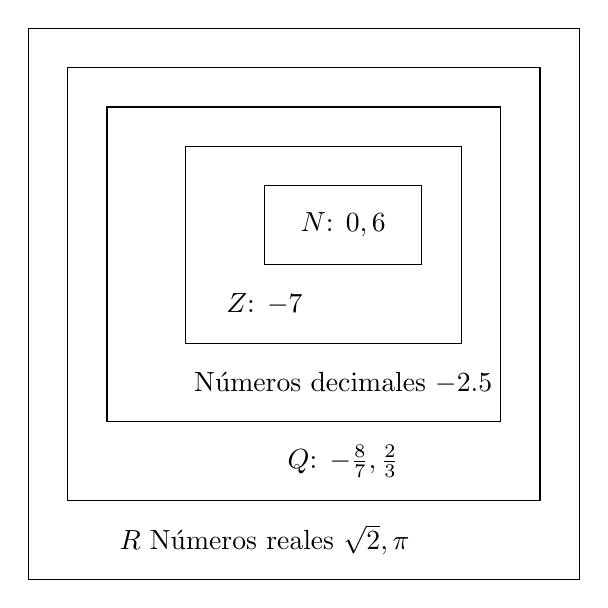
\begin{tikzpicture}
  \draw (0,0) rectangle(7,7);
  \path (3,0.5) node (R) {$\mathbb R$ Números reales $\sqrt{2}, \pi$};
  \draw (.5,1) rectangle(6.5,6.5);
  \path (4,1.5) node (Q) {$\mathbb Q$: $-\frac{8}{7}, \frac{2}{3}$};
  \draw (1,2) rectangle(6,6);
  \path (4,2.5) node (D) {Números decimales $-2.5$};
  \draw (2,3) rectangle(5.5,5.5);
  \path (3,3.5) node (Z) {$\mathbb Z$: $-7$};
  \draw (3,4) rectangle(5,5);
  \path (4,4.5) node (N) {$\mathbb N$: $0, 6$};
\end{tikzpicture}
\end{center}

\subsection*{Sequências}

Una sucesión es un conjunto de objetos unos detrás de otros, en un cierto orden.
Si la sucesión sigue para siempre, es una sucesión infinita, si no es una
sucesión finita. Los objetos de la sucesión son llamados los términos y
notados con un número natural en índice: $x_0, x_1, x_2, \ldots$. We give
some examples below. Note that we will often be interested in
sequências numéricas, where the terms are taken from one the conjuntos numéricos
previously mentioned.

\subsection*{Ejemplos}

\begin{itemize}
\item Eso es una sucesión finita de 5 simbolos:
  $s_0 = \square, s_1 = \triangle, s_1 = \diamond, s_3 = \blacksquare,
  s_4 = \blacktriangle$
\item Una palabra es una secuencia finita donde los términos son las letras.
\item El conjunto de los lenguages humanos no es una sucesión si ningún orden
  particular es dado.
\item Una secuencia de ADN o secuencia genética es una sucesión de letras en
  el conjunto  $\{ A, T, G, C \}$ en un cierto orden.
  Aunque pueda ser muy largo, es finita.
\item El conjunto de los enteros impares en el orden creciendo
  forma una sucesión
  infinita. Los términos son $I_n = 2n + 1$ para $n \in \mathbb N$.
\item El conjunto de posiciones de la piedra en la paradoja de la dicotomía de
  Zenón forma una sucesión infinita.
\begin{center}
 \begin{tikzpicture}
    \draw (0,0) --(10,0);
    \draw (0,-.2) --(0,0.2);
    \draw (10,-.2) --(10,0.2);
    \path (0,.5) node (0) {$0$};
    \path (10,.5) node (1) {$1$};

    \draw (5,-.1) --(5,0.1);
    \path (5,.5) node (p1) {$P_1$};

    \draw (7.5,-.1) --(7.5,0.1);
    \path (7.5,.5) node (p2) {$P_2$};

    \draw (8.75,-.1) --(8.75,0.1);
    \path (8.75,.5) node (p3) {$P_3$};

    \draw (9.375,-.1) --(9.375,0.1);
    \path (9.375,.5) node (etc) {$\ldots$};

    \draw (9.6875,-.1) --(9.6875,0.1);
    \draw (9.84375,-.1) --(9.8375,0.1);
  \end{tikzpicture}
\end{center}
\end{itemize}

\subsection*{Exercício 1}

Determinar los términos $x_n$ de esas secuencias y decir si son infinitivas.

\begin{enumerate}
\item $x_0 = 84$. Si $x_n$ es par, definimos $x_{n+1} = x_n / 2$ y si no nos
  paremos.
\item $x_0 = 2$. Si $x_n$ es par, definimos $x_{n+1} = x_n \times {(n+3)}$ y si
  no nos paremos.
\item $x_0 = 3$, $x_{n+1}$ es el resto de la división euclídea $2 x_n$ por 5 si
  es diferente de cero y si no nos paremos.
\item $x_0 = 3$, $x_{n+1}$ es el resto de la división euclídea $2 x_n$ por 12 si
  es diferente de cero y si no nos paremos.
\end{enumerate}

\subsection*{Exercício 2 (criba de Eratóstenes)}

Consideramos el conjunto de los números natural $\geq 2$. Eliminamos todos
los múltiplos de $2$ para formar el conjunto de números natural impar $\geq 3$.
El más pequeño número en este nuevo conjunto es $3$. Eliminamos todos
los múltiplos de $3$ para formar otro conjunto. En cada etapa, si queda un
conjunto que no es vacío, eliminamos los múltiplos del más pequeño elemento
en este conjunto y si no nos paremos aquí.

\begin{enumerate}
\item Describir los quatro primeros conjuntos obtenidos así.
\item Demostrar que cada conjunto en el orden creciente es una secuencia
  infinita (considerar $\{ p^n : n \in \mathbb N\}$ donde $p$ es el más
  pequeño elemento del conjunto).
\item Entonces obtenemos una secuencia de secuencias infinitas:
  $S_0, S_1, S_2, \ldots$. Muestrar que esa secuencia es infinita
  (si $p_n$ es el primer término de $S_n$, considerar
  $\left(p_0 \times p_1 \times \ldots \times p_n\right) + 1$).
\item Para $n \in \mathbb N$, consideremos $p_n$ es el primer término de $S_n$.
  ¿Que es la secuencia infinita $p_0, p_1, p_2, \ldots$?
\item Dar sus primeros términos (este algoritmo es llamado la criba de
  Eratóstenes).
\end{enumerate}

\section{Sucesiones aritméticas y geométricas}

\subsection*{Resumen}

Una sucesión aritmética (o progresión aritmética) es una sucesión
$u_0, u_1, u_2, \ldots$ de ńumeros en la que cada término permite deducir el
siguiente añadiendo una constante $k$, llamada diferencia común:

$$u_{n+1} = u_n + k$$

Entonces $u_0, u_1 = u_0 + k, u_2 = u_1 + k = u_0 + 2k,
u_3 = u_2 + k = u_0 + 3k$ y el término general es
%%
$$u_n = u_0 + {k n}$$

En una sucesión geométrica cada término se calcula multiplicando el anterior
por una constante $k$ denominada razón:

$$u_{n+1} = u_n \times k$$

Entonces $u_0, u_1 = u_0 \times k, u_2 = u_1 \times k = u_0 k^2,
u_3 = u_2 \times k = u_0 + k^3$ y el término general es
%%
$$u_n = u_0 k^n$$

\subsection*{Ejemplos}

\begin{enumerate}
\item $1, 4, 7, 10, 13, \ldots$ es una sucesión aritmética de diferencia común $3$.
  $u_0 = 1$ y $u_n = u_0 + 3n$.
\item $12, 6, 3, \frac{3}{2}, \frac{3}{4}, \frac{3}{8}, \ldots$ es sucesión
  geométrica de razón $\frac{1}{2}$. $u_0 = 12$ y
  $u_n = \frac{3}{2^{n-2}}$.
\item Si una secuencia empeza por
  $u_0 = 1, u_1 = 3, u_2 = 12$, tenemos $u_1 - u_0 = 2 \neq 9 = u_2 - u_1$ y
  $\frac{u_1}{u_0} = 3 \neq 4 = \frac{u_2}{u_1}$ entonces no puede ser ni
  una sucesión aritmética ni una sucesión geométrica.
\end{enumerate}

\subsection*{Exercício 3}

Indicar si las sucesiones siguientes son sucesión aritmética o geométrica y
dar la diferencia común / razón.

\begin{enumerate}
\item $-1, 1, -1, 1, -1, 1, \ldots$
\item $5, 2, -1, -4, -7, -10, -13, -16$
\item $\frac{50}{3}, 100, 600, 3600$
\item $1, 2, 4, 9, 16, 25, 36, \ldots$
\item La sucesión $x_n = n!$
\item La sucesión de los múltiplos de 7 más grande que 18.
\item La sucesión de los grados del polinomio $P_n$ donde
  $P_0 = X$ y $P_{n+1} = {(3X^2 - 1)} P_n$.
\item La sucesión del coeficiente principal de $P_n$.
\end{enumerate}

\section{Soma dos termos}

We can consider the soma dos $n$ primeiros termos $n$ $u_0, u_1, u_2, \ldots$
de uma sequência:

$$S_n = \sum_{i=0}^n u_i = u_0 + u_1 + u_2 + \ldots u_n$$

Si consideramos la sucesión de los $n$ primeros términos de una sucesión
aritmética, obtenemos una serie aritmética. Si consideramos la sucesión de los
$n$ primeros términos de una sucesión geométricas, obtenemos una serie
geométricas.

Si $u_0, u_1, u_2, \ldots$ es una sucesión aritmética de diferencia común $k$,
tenemos $u_0 + u_n = u_0 + u_0 + kn = 2u_0 + kn$ y de manera general, si
$0 \leq i \leq \frac{n}{2}$,
$u_i + u_{n-i} = u_0 + {in} + u_0 + {(n-i)}n = 2u_0 + kn = u_0 + u_n$.

$$
\begin{aligned}
2S_n &= \sum_{i=0}^n u_i + \sum_{i=0}^n u_{n-i}\\
     &= \sum_{i=0}^n \left(u_i + u_{n-i}\right) \\
     &= \sum_{i=0}^n {(u_0 + u_n)} \\
     &= {(n+1)}{(u_0 + u_n)}
\end{aligned}
$$

Finalmente
%%
$$
S_n = \frac{{(n+1)}{(u_0+u_n)}}{2} =
\frac{\text{número de términos} \times
\left(\text{primer término} + \text{último término}\right)}{2}
$$

Si $u_0, u_1, u_2, \ldots$ es una sucesión geométrica de diferencia razón $k$,
%%
$$
\begin{aligned}
k S_n &= k \left( u_n + \sum_{i=0}^{n-1} u_i \right)\\
      &= {k u_n} + \sum_{i=0}^{n-1} {k u_{i}} \\
      &= {k^{n+1} u_0} + \sum_{i=0}^{n-1} {u_{i+1}} \\
      &= k^{n+1} u_0 + S_n - u_0
\end{aligned}
$$

Entonces ${(k - 1)} S_n = {(k^{n+1} - 1)} u_0$. Además si $k=1$,
$u_n = u_0 1^n = u_0$ y $S_n = (n+1) u_0$. Finalmente
%%
$$
S_n =
\begin{cases}
{(n+1)} u_0 = \text{primer término} \times \text{número de términos}
& \text{si $k = 1$}; \\
u_0 \frac{k^{n+1} - 1}{k-1}
= \text{primer término} \times
\frac{\text{razón}^{\text{número de términos}} - 1}{\text{razón} - 1}
& \text{si $k \neq 1$}; \\
\end{cases}
$$

When $|k| < 1$, the formula becomes $S_n = u_0 \frac{1 - k^{n+1}}{1 - k}$.
But $k^{n+1}$ tends to $0$ when $n$ becomes large and so
$S_n$ tends to $\frac{u_0}{1-k}$. Hence we define
the infinite sum of the term to be:
%
$$
{\sum_{n=0}^{+\infty} u_n} = {u_0+u_1+u_2+\ldots} =
{u_0 \left(1 + k + k^2 + k^3 + k^4 + \ldots \right)} =
\frac{u_0}{1-k} =
\frac{\text{primer término}}{1 - \text{razón}} \; \text{si $|k| < 1$}
$$
%

\subsection*{Exercício 4}

Calcular

\begin{enumerate}
\item $5 + 7 + 9 + 11 + 13 + 15 + 17 + 19 + 21 + 23 + 25$
\item $-52 - 59 - 66 -73 - 80$
\item $-2 + 4 - 8 + 16 - 32 + 64$
\item El camino recorrido a la etapa $n$ de la paradoja de la dicotomía de
  Zenón. What is the total distance obtained by summing up the distance
  in each step?
\item $0.3333333\ldots = \frac{3}{10} + \frac{3}{100} + \frac{3}{100} +
  \frac{3}{1000} + \ldots = \sum_{n=1}^{+\infty} \frac{3}{10^n}$
\end{enumerate}

\subsection*{Exercício 5 (anécdota de Gaus)}

El maestro de escuela de Gaus propuso a sus alumnos de sumar los números de 1
a 100. Gaus dio la respuesta correcta casi inmediatamente.
Describe la sucesión y serie que aparacen en está anécdota y la respuesta
correcta.

\subsection*{Exercício 6 (fábula del Emperador chino y el ajedrez)}

``Como contrapartida de sus lecciones, el emperador de la China pide a un
maestro de ajedrez el regalo que quisiera.
El maestro pide que reciba la cantidad de arroz resultante de poner un grano en
la primera casilla, dos en la segunda, cuatro en la tercera, y así
sucesivamente.''

Describir el número de granos en las primeras casillas y indicar qué tipo
de sucesión encontramos? ¿Cual debería ser la cantidad de arroz en la decima
casilla? ¿En las quince primeras casillas?
La última casilla del tablero tendría 9223372036854775808 granos de arroz.
¿Determinar la cantidad de arroz total que el Emperador debería ofrecer?

\subsection*{Exercício 7 (Cantor Set)}

\begin{enumerate}
\item Given $C_0 = {[0,1]}$, we remove its open middle third segment
  $\left]\frac{1}{3},\frac{2}{3}\right[$ to obtain $C_1$.
  Express $C_1$ as the union of two disjoint segments.
\item  What is the set $C_2$
  obtained by removing the middle third of each of these two segments?
\item We continue like this to define $C_n$ obtained by removing middle
  thirds of each segments of $C_{n-1}$. Compare the terms of the sequence
  ${(C_n)}_{n \in {\mathbb N}}$ with respect to the inclusion of sets $\subset$.
\item Show that $C_n$ is a union of
  $2^n$ disjoint segments of length $\frac{1}{3^n}$.
  What is the length of $C_n$? What can you say about that
  sequence of lengths and its behavior when $n$ grows?
\item For each $n$ we define $X_n = C_n \setminus C_{n+1}$.
  Show that the sets $X_n$ are pairwise disjoint and express their lengths.
\item Let $C = {[0,1]} \setminus \left(\bigcup_{n=0}^{+\infty} X_n\right)$.
  What is the length of $C$?
\end{enumerate}

\section{Solução do Exercícios}

\subsection*{Exercício 1}

\begin{enumerate}
\item Finita secuencia: $x_0 = 84, x_1=42, x_2 = 21$.
\item $x_0 = 2$. $x_0$ es par entonces definimos $x_1 = 2 \times {(0+3)} = 6$.
  $x_1$ es par, definimos $x_2 = 6 \times {(1+3)} = 24$. De manera general,
  nos damos cuenta que los términos siempre son pares y entonces la secuencia
  es infinitivas de término $x_n = {(n+2)}! =
  {(n+2)} \times {(n+1)} \times n \times \ldots \times 2$.
\item $x_0 = 3$. $2 x_0 = 6 = 5 \times 1 + 1$ entonces $x_1 = 1$.
  $2 x_1 = 2 = 5 \times 0 + 2$ entonces $x_2 = 2$.
  $2 x_2 = 4 = 5 \times 0 + 4$ entonces $x_3 = 4$.
  $2 x_3 = 8 = 5 \times 1 + 3$ entonces $x_4 = 3 = x_0$.
  $2 x_4 = 6 = 5 \times 1 + 1$ entonces $x_5 = 1 = x_1$. Nos damos cuenta de
  que es una secuencia infinita formada por la repetición de los cuatro primeros
  términos: $3,1,2,4,3,1,2,4,3,1,2,4,3,1,2,4\ldots$.
\item $x_0 = 3$. $2 x_0 = 6 = 12 \times 0 + 6$ entonces $x_1 = 6$.
  $2 x_1 = 12 = 12 \times 1 + 0$ entonces nos paremos. La secuencia es finita
  con dos términos: $x_0=3, x_1=6$.
\end{enumerate}

\subsection*{Exercício 2}

\begin{enumerate}
\item El primer conjunto es el conjunto de los números naturales $\geq 2$
  $\{ 2, 3, 4, 5, 6, \ldots \}$, el segundo
  es el conjunto de números natural impar $\geq 3$: $\{ 3, 5, 7, 9, 11, \ldots \}$.
  El tercero es el conjunto de números natural impar que no son múltiplos de
  3: $\{ 5, 7, 11, 13, \ldots \}$. $5$ es el más pequeño elemento entonces
  el cuarto conjunto es el conjunto de números natural que no son múltiplos de
  2, 3, o 5: $\{ 7, 11, 13, 17, 19, \ldots \}$.
\item Solo necesitamos que mostrar que los conjuntos son infinitivos y
  considerando el ordern de los número naturales, obtenemos una secuencias
  infinitas. Ya hemos visto que los primeros conjuntos son infinitivos.
  Si un conjunto no es vacío, su más pequeño elemento $p$ no es un múltiplo
  de los más pequeño elementos $2, 3, 5, 7, \ldots$ de los conjuntos precedentes y
  entonces eso es también verdad para $p^2, p^3, p^4, \ldots$. Entonces esos
  números no han sido eliminados y aún se queda una infinidad de números.
\item Para etapa $n \in \mathbb N$ por la que el conjunto no es vacío,
  el número $\left(p_0 \times p_1 \times \ldots \times p_n\right) + 1$)
  no es múltiplo de cada $p_0, p_1, \ldots, p_n$ y entonces no es eliminado durante
  las etapas $0, 1, 2, \ldots, n$. Como consecuencia, el conjunto a la etapa
  $n+1$ no es vacío y podemos definir la secuencia $S_{n+1}$.
\item Por construcción, son los números que solo son múltiplos 1 o ellos mismos,
  es decir los número primos.
\item $p_0=2, p_1=3, p_2=5, p_3=7, p_5=11, p_6=13, p_7=17, p_8=19$.
\end{enumerate}

\subsection*{Exercício 3}

Indicar si las sucesiones siguientes son sucesión aritmética o geométrica y
dar la diferencia común / razón.

\begin{enumerate}
\item Sucesión geométrica de razón $-1$.
\item Sucesión aritmética de diferencia común $-3$.
\item Sucesión geométrica de razón $6$.
\item Ni geométrica ni aritmética. $u_2 - u_1 = 2 \neq 1 = u_1 - u_0$ y
  $\frac{u_2}{u_1} = 2 \neq 2.25 = \frac{u_3}{u_2}$.
\item Ni geométrica ni aritmética. $x_1 - x_0 = 0 \neq 1 = x_2 - x_1$
  y $\frac{x_2}{x_1} = 2 \neq 1 = \frac{x_1}{x_0}$.
\item $21, 28, 35, 42, \ldots$ es una sucesión geométrica de razón $7$.
\item $P_0 = X$, $P_1 = 3X^3 - X$, $P_2 = 9X^5-6X^3+X$,
  $P_3 = 27X^7-27X^5+9X^3-X$. De manera general, vemos que $P_n$ es de grado
  $x_=2n+1$ entonces esos grados forman una sucesión aritmética de
  diferencia común $2$.
\item De manera general, vemos que el coeficiente principal de $P_n$ es
  $3^n$ entonces esos coeficientes forman una sucesión geométrica de
  razón $3$.
\end{enumerate}

\subsection*{Exercício 4}

\begin{enumerate}
\item Reconocimos una sucesión aritmética de diferencia común 2 y obtenemos
  $11 \times \frac{5 + 25}{2} = 11 \times 15 = 165$.
\item Reconocimos una sucesión aritmética de diferencia común $-7$ y obtenemos
  $5 \times \frac{-52 + -80}{2} = 5 \times -66 = -330$
\item Reconocimos una sucesión geométrica de razón $-2$ y obtenemos
  $-2 \times \frac{{-2}^{6} - 1}{-2 - 1} = \frac{2}{3} \times 63 = 42$
\item El camino recorrido $d_1, d_2, \ldots$ durante cada etapa es
  $d_n = \frac{1}{2^n}$. Es una sucesión geométrica de razón $\frac{1}{2}$. El
  camino recorrido total a la etapa $n$ es
  $$
  S_n = \sum_{i=1}^n d_i = \frac{1}{2} \times \frac{\left(\frac{1}{2}\right)^n - 1}{\frac{1}{2} - 1} = 1 - \frac{1}{2^n}
  $$
  The total distance is of course the length of the whole $[0,1]$ segment:
  $$
  \sum_{i=1}^{+\infty} d_i = \frac{1}{2} \frac{1}{1 - \frac{1}{2}} = 1
  $$
\item This is the infite sum of the terms of a geometric sequence of
  ratio $\frac{1}{10} < 1$. Hence
  $0.3333333\ldots = \frac{3}{10} \frac{1}{1-\frac{1}{10}} =
  \frac{3}{10} \frac{10}{9} = \frac{1}{3}$.
\end{enumerate}

\subsection*{Exercício 5 (anécdota de Gaus)}

Vemos una sucesión aritmética $u_n = n$ de primer término $u_1 = 1$ y de
diferencia común $1$. La suma que calcular es la serie de los 100 primeros
términos:

$$
S_{100} = \frac{{100} \times {(1+100)}}{2} = 50 \times 101 = 5050
$$

\subsection*{Exercício 6 (fábula del Emperador chino y el ajedrez)}

Hay $x_1=1$ grano en la primera casilla, $x_2=2$ en la segunda, $x_3=4$ en la
tercera y $x_4=8$ en la cuarta. Eso es una sucesión geométrica de razón $2$.
El término general est $x_n = 2^{n-1}$ y entonces la
cantidad de arroz en la decima casilla es $x_{10} = 2^{10-1} = 512$ granos.

El término general para la cantidad en los $n$ primeras casillas es
$S_n = \sum_{i=1}^n x_i = x_1 \frac{2^n-1}{2-1} = 2^n - 1$. Entonces,
la cantidad de arroz en las quince primeras casillas es
$S_{15}  = 2^{15} - 1 = 32767$.

La última casilla del tablero tiene
$x_{64} = 9223372036854775808 = 2^{63}$ granos. Entonces la cantidad total de
arroz es $S_{64} = 2^{64} - 1 = 2 \times 2^{63} - 1 =
2 \times 9223372036854775808 - 1$. Podemos efectuar esta operación y obtenemos
$S_{64} = 18446744073709551615$.

\subsection*{Exercício 7 (Cantor Set)}

\begin{enumerate}
\item $C_1 = \left[0,\frac{1}{3}\right] \cup \left[\frac{2}{3},1\right]$.
\item $C_2 = \left[0,\frac{1}{9}\right] \cup
  \left[\frac{2}{9},\frac{1}{3}\right]
  \cup \left[\frac{2}{3},\frac{5}{9}\right] \cup \left[\frac{8}{9},1\right]$.
\item $C_{n+1}$ is obtained by removing elements from $C_n$ so we have a
  decreasing sequence $C_0 \supset C_1 \supset C_2 \supset C_3 \supset \ldots$.
\item
  This is indeed true for $C_0$ and $C_1$ and $C_2$. If this is true
  for $C_n$ then each of the $2^n$ segments is splitted into three parts
  and we keep $2$ of these parts. Hence the number of segments doubles
  while their length is divided by three. Hence $C_{n+1}$ is made of
  $2 \times 2^n = 2^{n+1}$ segments of length $\frac{\frac{1}{3^n}}{3} =
  \frac{1}{3^{n+1}}$ and so the expression is true for $C_{n+1}$ too.

  We deduce that the length of $C_n$ is
  $2^n \times \frac{1}{3^n} = \left(\frac{2}{3}\right)^n$.
  This sequence of lengths is then geometric of ratio $\frac{2}{3}$. The
  lengths decrease and tend to $0$ when $n$ grows.
\item $X_n$ corresponds to the numbers removed from $C_n$ to obtain
  $C_{n+1}$ and so the $X_n$'s are indeed disjoint (we can not remove again
  what has already been removed!).
  $C_{n+1}$ is of length $\left(\frac{2}{3}\right)^{n+1}$,
  $C_n$ is of length $\left(\frac{2}{3}\right)^{n}$ and we have
  $C_{n+1} \subset C_n$. Hence the length of $X_n$ is
  $\frac{2^n}{3^n} - \frac{2^{n+1}}{3^{n+1}} =
  \frac{{(3 - 2)} \times 2^n}{3^{n+1}} = \frac{1}{3} \left(\frac{2}{3}\right)^n$
\item The $X_n$ are disjoints of length $\frac{1}{3} \left(\frac{2}{3}\right)^n$
  by the previous question. We recognize a geometric sequence of ration
  $\frac{2}{3}$ and so the length of $\bigcup_{n=0}^{+\infty} X_n$ is
  %
  $$\sum_{n=0}^{+\infty} \frac{1}{3} \left(\frac{2}{3}\right)^n =
  \frac{1}{3}\frac{1}{1-\frac{2}{3}} = 1$$
  %
  The length of $[0,1]$ is $1$ and so the length of $C$ is $1 - 1 = 0$.
\end{enumerate}
